\documentclass[12pt,oneside,english]{article}

\usepackage[T1]{fontenc}
\usepackage[latin1]{inputenc}
\usepackage{geometry}
\geometry{verbose,letterpaper,tmargin=1in,bmargin=1in,lmargin=1in,rmargin=1in}
\usepackage{textcomp}
\usepackage{babel}
\setcounter{secnumdepth}{0}
\usepackage{graphicx}
\usepackage{float}
\floatstyle{boxed}
\restylefloat{figure}
\usepackage{longtable}
\usepackage{url}

\usepackage{listings}
\usepackage{color}

\definecolor{mygray}{rgb}{0.4,0.4,0.4}
\definecolor{mygreen}{rgb}{0,0.8,0.6}
\definecolor{myorange}{rgb}{1.0,0.4,0}

\lstset{language=Matlab,
   keywords={break,case,catch,continue,else,elseif,end,for,function,
      global,if,otherwise,persistent,return,switch,try,while},
   basicstyle=\sffamily,
   keywordstyle=\color{blue},
   commentstyle=\color{dkgreen},
   stringstyle=\color{red},
   numbers=left,
   numberstyle=\tiny\color{gray},
   stepnumber=1,
   backgroundcolor=\color{white},
   tabsize=4,
   showspaces=false,
   showstringspaces=false}
\lstset{
basicstyle=\footnotesize\sffamily\color{black},
commentstyle=\color{mygray},
frame=single,
numbers=left,
numbersep=5pt,
numberstyle=\tiny\color{mygray},
keywordstyle=\color{mygreen},
showspaces=false,
showstringspaces=false,
stringstyle=\color{myorange},
tabsize=4
}

\newcommand{\BibTeX}{{\sc Bib}\TeX}


\begin{document}

\title{In-Situ Impedance Measurement and Size Analysis of Multi-Layer Assembled Gold Nano-Island Film}

    \author{John Donovan, Dr. Chuhee Kwon\\
    University of California, Long Beach, CA\\
    {\small donovan.csulb@gmail.com ckwon@csulb.edu}}
    
        \date{\today}

\abstract{
    On a self-assembled multi-layer film, gold particles are deposited layer by layer on a substrate, using organic molecules to mediate the deposition.
    The organic molecules burn off at high temperatures (thermolysis), and this breakdown deposits the gold into a single layer.
    Gold nanoislands aggregate during annealing.
    The impedance of the nano-island and substrate may be measured during this heating, and phase transitions may be observed.
    The analysis of resulting nano-island samples is derived from Atomic Force Microscope images -- the sparse islands benefit from a ``blob finder'' approach using computer vision libraries and analysis that measures cross-sections.
}

    \maketitle

    \tableofcontents

\section{SCOPE}
    This document is a discussion of the Spring 2012 End-of-Semester summary slides, presented to the CSULB Department of Physics and Astronomy on May 7th 2012.
    The summary slides describe the process of in-situ impedance measurements, experimental uncertainty thereof, and present the measured impedance for sparse islands and bare glass.


\section{INTRODUCTION}

Rubinstein characterized morphology and spectral absorption of nanoislands formed by annealing evaporated gold films \cite{doron2004}.


\section{TESTBED HARDWARE}
    \subsection{Self-Assembling Multilayer Film Wet Chemistry Station}
        A wet chemistry station was set up for the creation of multilayer nanoisland slides.  

    \subsection{In-situ impedance measurement thermolysis and annealing station}
        A sketch was written in NI LabView to monitor temperatures and Impedance measurements.  
        A lab furnace used for thermolysis and annealing was customized with temperature control and measurement electronics.  

        \subsection{Atomic Force Microscope and Scanning Electron Microscope}


        \subsection{Analysis and Image Processing Workstation}


\section{TEMPERATURE CONTROL, MEASUREMENT AND ERRORS}

    In-situ measurements require the accurate measurement of temperature and impedance.  
    The impedance is measured at the sample, while the temperature is inferred from thermocouple measurements.
    
    \subsection{Shortcomings in Oven Temperature Measurement}
        
    Temperature measurements with more than one thermocouple showed that fast heating is uneven across the furnace.  
    Also, during fast heating, impedance measurements of a bare electrode did not match their expected temperature dependants, 
    when the temperature was measured with a nearby 10-mil bare wire K-type thermocouple in air.
    The glass of the electrode caused the sample temperature to lag up to $100^{\circ}C$ behind the air temperature during fast heating (Figure ~\ref{f:bare_vs_glass}).

    \subsection{Temperature Controller}
    [ Link to the Appendix TBD: Temperature Controller Schematics, BOM, and Code]
    An automated PID controller was constructed using Arduino microcontroller, a thermocouple daughter-board, and the existing solid-state relay within the Thermolyne furnace.  

    [ Link to the Appendix TBD: Temperature Controller Schematics, BOM, and Code]
    
    \subsubsection*{Temperature Control Requirements}    
    To allow temperature to be accurately measured (within $50^{\circ}C$ or better) during fast heating, the heating rate must be controlled during heating.
    The COTS Thermolyne furnace temperature controller is a simple PID, which when given a setpoint temperature, will approach this temperature as fast as its capabilities allow.
    To slow the heating to a rate such that the sample temperature may be accurately measured during heating, the PID setpoint was a time-varying function that ramps to the final temperature.

    Prior experiments by Toyanath Joshi used a methodical and manual approach of increasing the PID setpoint temperature at the desired rate.  

    The controller was run through some heating cycles to determine the maximum rate for reliable heating, and which of several thermocouples should be used for (1) control, and (2) the sample temperature.
    
    \subsubsection*{Temperature Controller}

    For the research conducted here, an automated PID controller was constructed using Arduino microcontroller, an open-source hardware thermocouple add-on, and the existing solid-state relay within the Thermolyne furnace.  
    The Arduino microcontroller is well-documented (cite:arduino.cc), and its form factor supports a number of add-on boards(``shields'') produced by a large number of independant amateur and commercial vendors.
    The thermocouple ``shield'' contains four addressable MAX31855 thermocouple digitizers with cold-junction compensation and includes connectors for four K-type thermocouples.
    The solid-state relay within the Thermolyne furnace was disconnected from the old PID control and connected to the output pin (pin 7) of the new controller.

    The Arduino has a USB computer interface but also runs stand-alone code independently of the computer.
    This means the oven temperature is always controlled by the microcontroller, but the computer interface may be used to request changes to the program running on the controller.
    The computer is used to set a final setpoint temperature and a rate at which the temperature should be approached.  
    The microcontroller uses these two parameters, along with the current temperature measured from its sensor, to break the ramp into a time-dependant setpoint temperature to pass to a PID algorithm.
    The PID algorithm decides how best to approach the current setpoint (which will change over time), and over time, the final setpoint will be reached.

    [the PID is better described by code or flow chart than equation]
    


    In the temperature controller designed here, any single one of four thermocouples can be used in the PID controller.	  
    Bare thermocouples, the oven's existing thermocouple, and a thermocouple bonded to a glass slide were each measured during oven heating.
    
    

    \subsection{Temperature Measurement}
    
    \begin{figure}
    	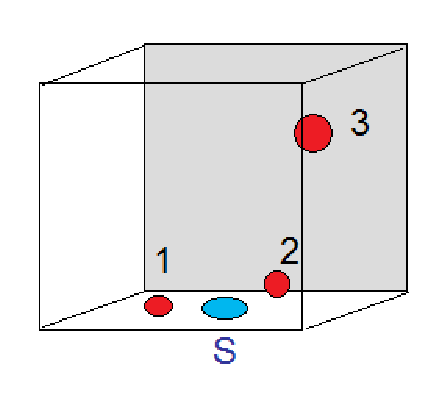
\includegraphics[width=70mm]{images/oven_tc_placement.eps}
    	\caption{Placement of the three thermocouples and the sample within the furnace used to measure furnace/sample temperature.  TC \#1 is the glass-slide thermocouple, TC \#2 is a bare TC, TC \#3 is the furnace TC, and ``S'' is the sample.}
    	\label{f:furnace_tc}
    \end{figure}
    
    \begin{figure}
    	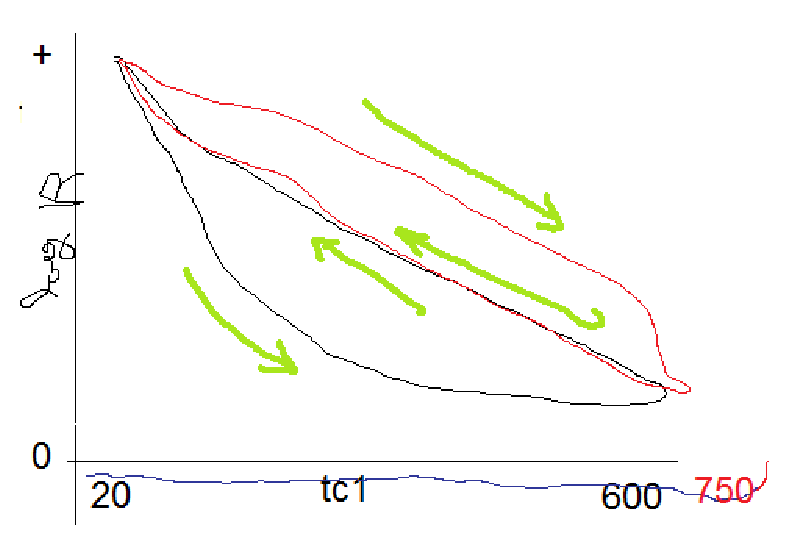
\includegraphics[width=150mm]{images/plot_logR_vs_tc1_and_tc3.eps}
    	\caption{Placeholder for missing graphic.  If temperature is accurately measured, the log impedance of the bare IDE sample will match on heating and cooling.  If the thermocouple temperature heats faster than the sample, the sample resistance will appear higher on (fast) heating than (slow) cool-down (red trace).  If the thermocouple temperature lags the sample temperature on heating, the sample resistance will appear lower on heating than cool-down (black trace).  The closer the overlap between heating and cooling, the better the thermocouple matches the temperature seen by the sample. }
    	\label{f:logR_vs_t1_and_t3}
    \end{figure}
    
    \begin{figure}
    	\includegraphics[width=150mm]{images/oven_heating_bare_vs_glass_tc.eps}
    	\caption{The temperature difference measured between a bare thermocouple and thermocouple attached to a glass slide with silver epoxy shows the bonded thermocouple is slower to heat and cool.  The temperature difference can exceed 100$^{\circ C}$.}
    	\label{f:bare_vs_glass}
    \end{figure}

    Use of multiple thermocouples (Figure ~\ref{f:furnace_tc}) to measure furnace temperature during very rapid heating showed large temperature gradients within the furnace, and that the glass slides on which the samples are mounted slow the heating of the sample.

    Three thermocouples were used to measure furnace temperature.  
    The furnace has a heavy gauge K-type thermocouple at the top of the furnace (tc3 in Figure ~\ref{f:furnace_tc}).  
    A bare 10 mil ($254{\mu}m$) thermocouple (tc2 in Figure ~\ref{f:furnace_tc}) was situated near the bottom of the furnace.  
    A third thermocouple (tc1 in Figure ~\ref{f:furnace_tc}) was attached to a glass microscope slide with a dab of silver epoxy and placed next to the sample.
    
    The IDE sample is responsive to temperature, and a bare IDE should show the same impedance during (fast) heating as it shows during (slow) cooling (Figure ~\ref{f:logR_vs_t1_and_t3}).  
    If the temperature measured by a thermocouple results poor overlap of the IDE impedance on the heating and cooling phases, a temperature error can be inferred.
    In this way the bare slide can serve as a fourth temperature-sensitive device to confirm that the "sample temperature" inferred from the thermocouple temperature measurements accurately tracks temperature.  
    
    The furnace PID controller creates a closed-loop temperature control system, using a single thermocouple to measure the furnace temperature, and a solid-state relay to turn the furnace on and off. 

    In the modified temperature controller, any thermocouple can be used in the PID controller.	
    
    For all furnace tests in Spring 2012, we selected a thermocouple mounted to a glass slide by silver epoxy to close the loop of the PID system.
    Since the glass-slide TC best tracks the temperature of the IDE sample, it was believed to result in fastest heating.
    However, because the glass is slower to heat than the air, it can cause a situation in which the furnace overheats. 
    
    It was discovered in early testing that the glass slide IDE lags behind the temperature at the top of the furnace by as much as $200^{\circ}C$ during fast heating of $30^{\circ}C/min$ (Figure ~\ref{f:bare_vs_glass}).  
    The build-up of heat and the lag of the glass TC resulted in an overheating of the oven when there is no additional safety measures.  
    A safety measure was introduced into the furnace controller code to turn off the heat if any TC measured greater than $+50^{\circ}C$ from the furnace setpoint.

\subsection*{Results of Thermocouple Selection}
    For all furnace tests in Summer 2012, we selected a bare thermocouple positioned at the bottom of the furnace (tc2 in Figure ~\ref{furnace_tc}) to close the loop of the PID system.
    Use of the bare TC in the PID system avoids the problem of overheating, and in testing (Section ~\ref{sec:Temperature_Uniformity_Three_Slides}), the glass slide temperature was controlled under fast heating to $625^{\circ}C$ at a rate of $30^{\circ}C/min$ with an overshoot of the sample temperature (measured by the glass slide) of just $2^{\circ}C$  [TBR].  
    The lack of run-away heating results from the rapid response of the glass slide thermocouple to small changes in air temperature within the furnace, and the mass of the glass slide which causes a slow approach to the final temperature.

    
    \subsection{Temperature Errors: Fast Heating is Uneven} \label{sec:Temperature_Uniformity_Three_Slides}

    \subsubsection{Analysis of Furnace Temperature Uniformity Using Three Glass Slide Thermocouples}

    \begin{figure}
    	\includegraphics[width=140mm]{images/Oven_Thermocouple_4x.eps}
    	\caption{Additional glass slide thermocouples were produced and used to measure the uniformity of the furnace temperature and similarity among glass-slide thermocouples.  Three glass slide thermocouples were used for measurement, and a fourth bare TC was used in the PID controller during this test.}
    \end{figure}
    \begin{figure}
    	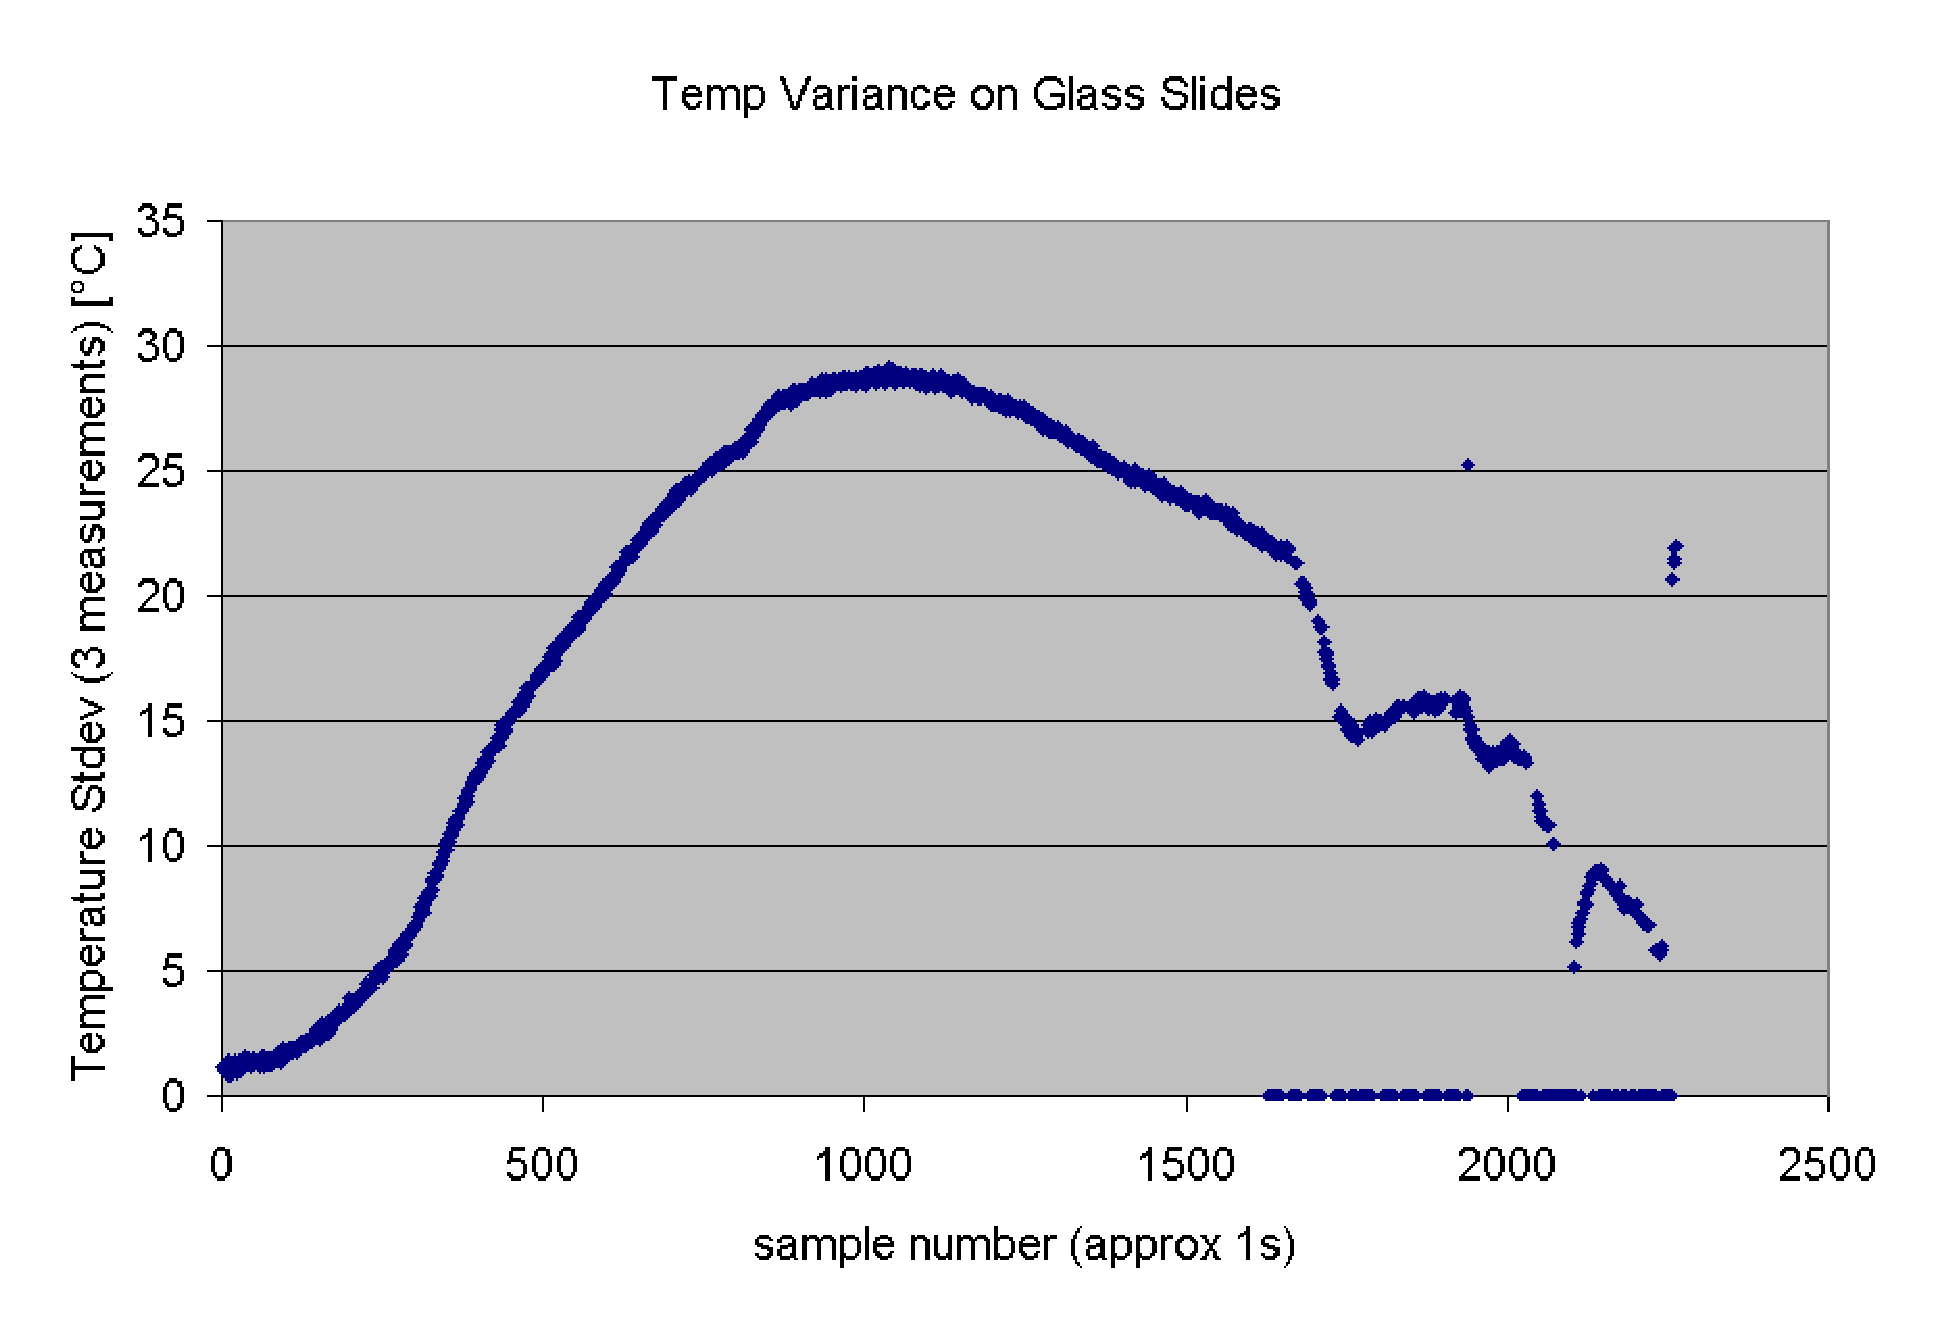
\includegraphics[width=140mm]{images/heating_data.eps}
    	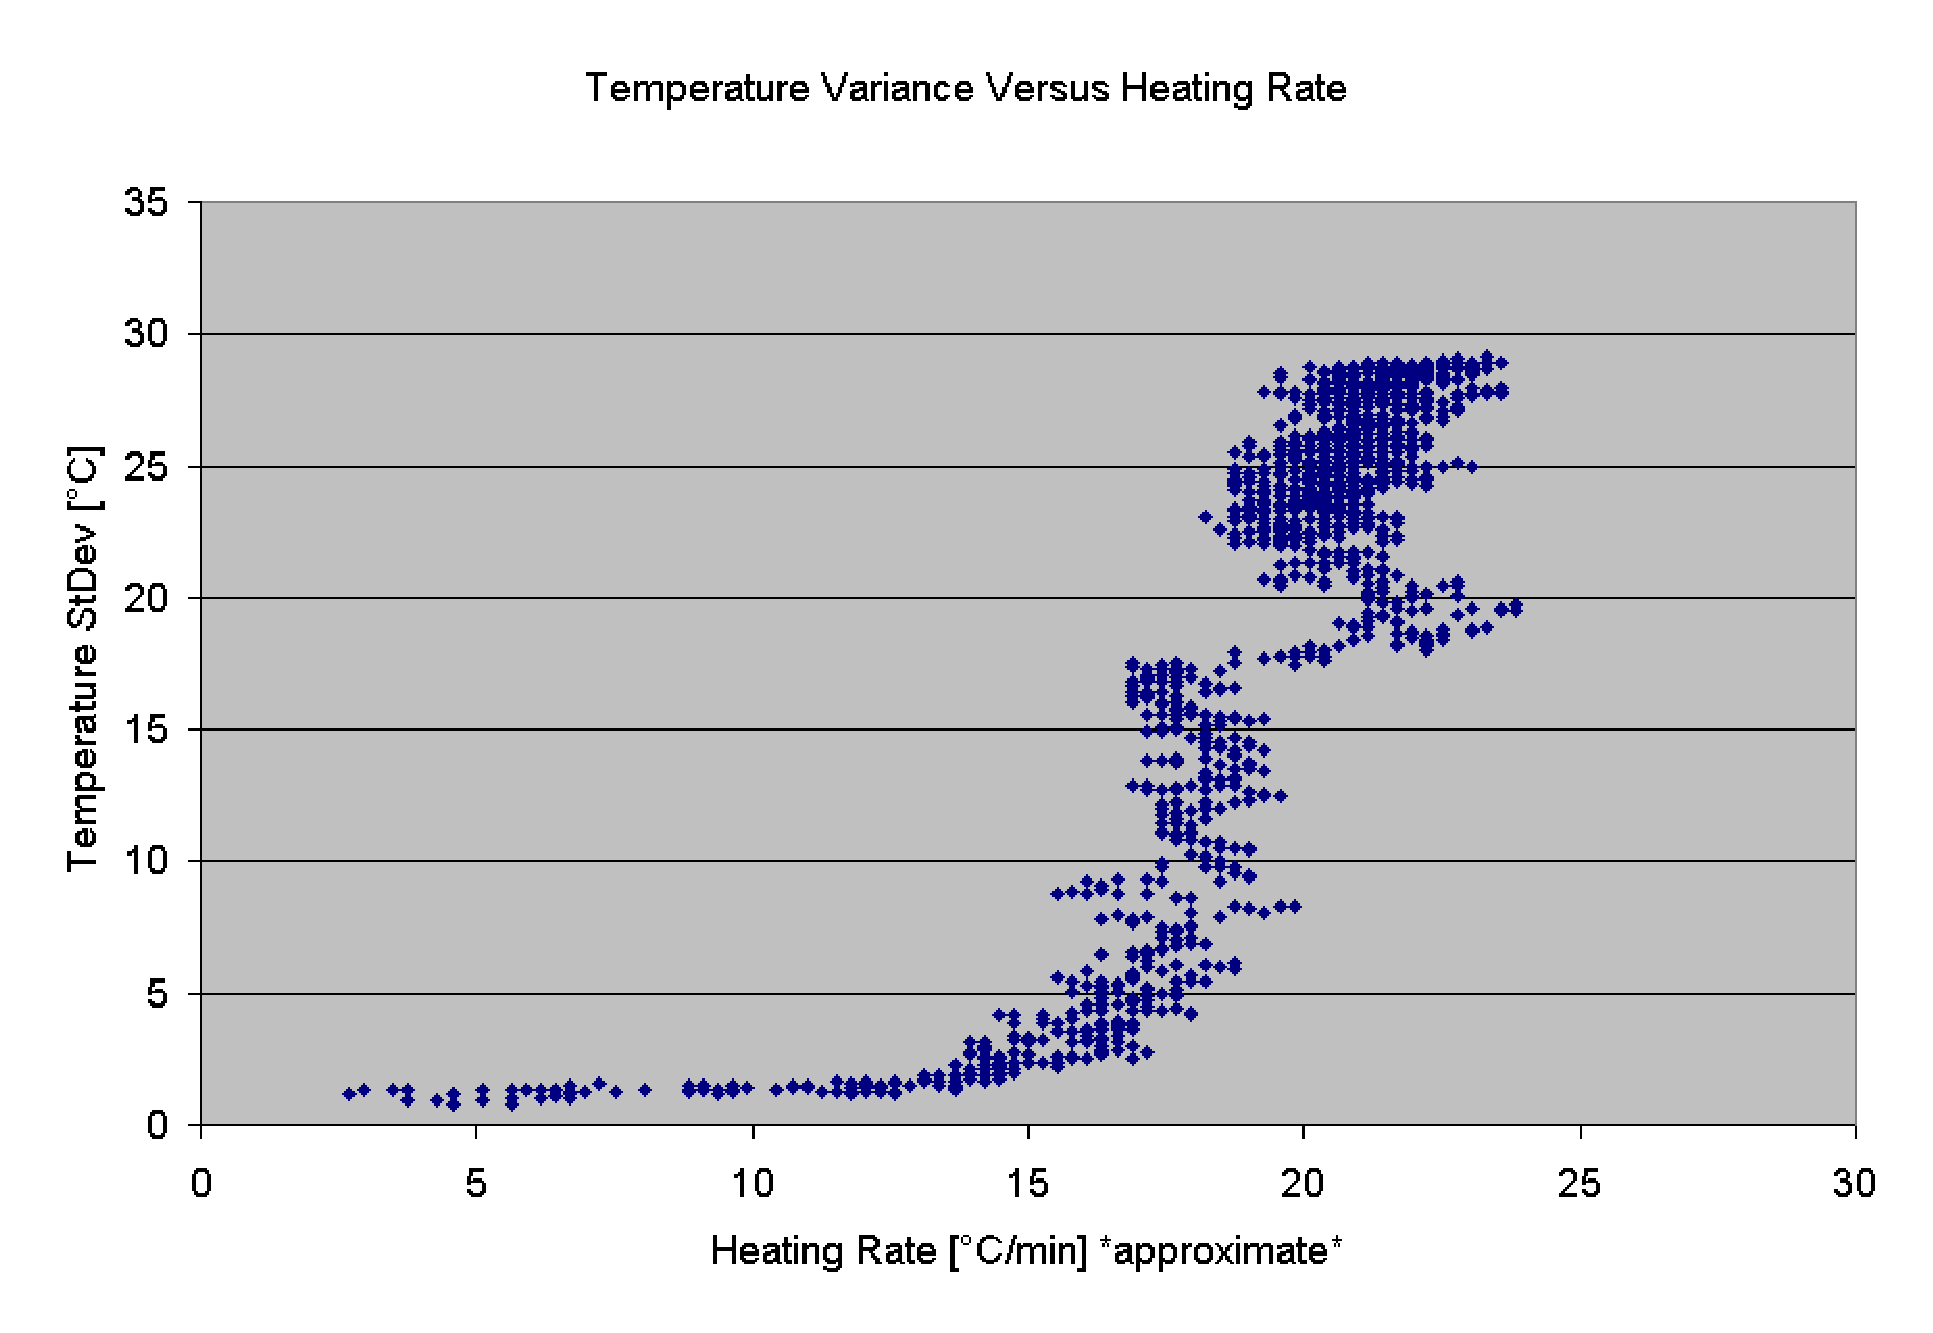
\includegraphics[width=140mm]{images/variance_vs_rate.eps}
    	\caption{The plot at left shows the standard deviation among the three glass slide thermocouples during fast heating, which is approximately the magnitude of the bias uncertainty in temperature during heating.  The temperature variance versus heating rate is plotted at left.  The magnitude of the temperature gradients across the base of the furnace are non-linearly proportional to temperature.}
    \end{figure}
    
    To test the reproducibility of the glass slide thermocouple, three glass slide thermocouples were made, by affixing a K-type thermocouple to the surface of a glass microscope slide.
    A fourth thermocouple was left bare and placed at the bottom of the furnace for use in the PID temperature controller.
    While the glass slide thermocouple can be used in the PID loop to raise the furnace temperature, it requires a gradient limiter to function safely.  
    The gradient limiter shuts off heating if the temperature between any two thermocouples exceeds a threshold ($50^{\circ}C$ was used), and is best used with one thermocouple at the top of the furnace (otherwise the gradient is not well sampled).

    Because the temperature controller built for this project is limited to four K-type thermocouples, a trade-off was made between fast heating (for which a glass slide TC is used) and complexity (the requirement that the heating gradient be limited). 
    A consequence to using an furnace shut-off is that the heating is no longer at an even rate, and the temperature characterization emphasizes errors (Figure "shutoff emphasizes errors in Au25 test").

    Results of the glass slide thermocouple uniformity measurement shows that three glass slides placed across the bottom of the furnace, when heated at a rate $25^{\circ}C$ per second, show a disagreement of $TBR^{\circ}C$ at the fastest rate of heating (Figure "three slides result").

\section{APPENDIX: ARDUINO}

\lstset{caption=Temperature Control Functions, label=lst:arduRelay}
\lstinputlisting[language=C++]{./_code/tc_relay_control.ino}

\lstset{caption=Arduino PID Controller v1 Library, label=lst:arduPid}
\lstinputlisting[language=C++]{./_code/PID_v1.cpp}


\bibliography{thesis_draft}
\bibliographystyle{plain}

\end{document}
